\documentclass[12pt]{article}



\usepackage{amsmath, amsthm, amssymb, amsfonts}
\usepackage{mathtools}
\usepackage{thmtools}
\usepackage{etoolbox}
\usepackage{enumerate, enumitem}
\usepackage{tikz}
\usepackage[dvipsnames]{xcolor}
\usepackage[framemethod=TikZ]{mdframed}


\def\theenumi{(\arabic{enumi})}
\def\thefootnote{(\arabic{footnote})}



\def\R{\mathbb{R}}
\def\Q{\mathbb{Q}}
\def\Z{\mathbb{Z}}
\def\N{\mathbb{N}}

% ==> Definition
\mdfdefinestyle{mdDefinitionStyle}{
  % roundcorner       = 0pt,
  % linewidth         = 0.8pt,
  skipabove         = 12pt,
  innerbottommargin = 9pt,
  skipbelow         = 2pt,
  nobreak           = false,
  % linecolor         = Gray,
  % backgroundcolor   = TealBlue!8,
}
\declaretheoremstyle[
  headfont      = {\sffamily\bfseries},
  bodyfont      = {\normalfont},
  mdframed      = {style=mdDefinitionStyle},
  headpunct     = {\\[3pt]},
  postheadspace = {0pt},
  notefont      = {\normalfont\sffamily\small},
  notebraces    = {~(}{)},
]{mdDefinition}

% ==> Theorem
\mdfdefinestyle{mdTheoremStyle}{%
  % linewidth           = 1pt,
  skipabove           = 12pt,
  frametitleaboveskip = 5pt,
  frametitlebelowskip = 0pt,
  skipbelow           = 2pt,
  innertopmargin      = 5pt,
  innerbottommargin   = 8pt,
  nobreak             = false,
  % linecolor           = Gray,
  % backgroundcolor     = Apricot!10,
}
\declaretheoremstyle[
  headfont      =\bfseries\sffamily,
  headindent    =0pt,
  bodyfont      =\itshape,
  mdframed      ={style=mdTheoremStyle},
  notefont      =\normalfont\sffamily\small,
  notebraces    = {~(}{)},
  headpunct     ={\(:\) },
  postheadspace ={2pt},
]{mdTheorem}



\declaretheorem[style=mdDefinition, name={Definition}, ]{definition}
\declaretheorem[style=mdTheorem, name={Theorem}]{theorem}
% \declaretheorem{example}[name={\exampleName},style=mdExample, numberwithin=chapter]
% \declaretheorem{exercise}[name={\exerciseName},style=mdExercise, numberwithin=chapter]

\theoremstyle{definition}
\newtheorem{exercise}{Exercice}
\newtheorem{example}{Example}



\renewcommand\epsilon{\varepsilon}
\def\R{\mathbb{R}}
\def\Q{\mathbb{Q}}
\def\Z{\mathbb{Z}}
\def\N{\mathbb{N}}
\mathtoolsset{centercolon} % not work when using |mathpazo|
\DeclarePairedDelimiter\abs{\lvert}{\rvert}
\DeclarePairedDelimiter\floor{\lfloor}{\rfloor}
\DeclarePairedDelimiterX\norm[1]\lVert\rVert{
	\ifblank{#1}{\:\cdot\:}{#1}
}



\usepackage{geometry} %[showframe]
\geometry{
  top=25.4mm,         % 1 inch
  bottom=41mm,        % 1.618 inches
  left=38mm,          % 1.5 inches
  right=38mm,         % 1.5 inches
}

% \geometry{
%   top=25.4mm,         % 1 inch
%   bottom=41mm,        % Golden ratio for bottom margin
%   inner=25.4mm,       % Smaller inner margin (1 inch)
%   outer=41mm,         % Larger outer margin (Golden ratio: 1.618 inches)
%   bindingoffset=10mm  % Optional space for binding (adjust as needed)
% }



% \newcounter{tdcounter}
\newcommand{\tdtitle}[2]{
  \noindent\rule{\textwidth}{0.8pt}
  \flushleft
    {\slshape Royal University of Phnom Penh \hfill Elementary Real Analysis}\\
    {\slshape Undergraduate Mathematics \hfill Class of 2024-2025}
  \endflushleft
  
  \vspace{0.8mm}
  \center
  {\sffamily\large TD n\textdegree #1 ~\textendash~ #2}
  \endcenter
  \noindent\rule{\textwidth}{0.8pt}
}



% \renewcommand{\qedsymbol}{\(\blacksquare\)}
\makeatletter
\renewenvironment{proof}[1][\proofname]{\par
  \pushQED{\qed}%
  \normalfont \topsep6\p@\@plus6\p@\relax
  \trivlist
\item\relax
  {\sffamily #1\@addpunct{.}}\hspace\labelsep\ignorespaces
}{%
  \popQED\endtrivlist\@endpefalse
}
\makeatother

\title{Elementary Real Analysis}
\author{\textsc{Sivmeng HUN}}
\date{32 Novembre 2024}

\usepackage{hyperref}


\begin{document}
\maketitle

\section{What is the set \(\R\)?}
In this lecture, we assume there are sets
\begin{align*}
  \N &= \{ 1, 2, 3, \dots\}\\
  \Z &= \{ 0, \pm 1, \pm 2, \dots\}\\
  \Q &= \{\tfrac{p}{q}\colon p\in\Z,~ q\in\N\}.
\end{align*}
Moreover, we assume there is another \(\R\) that is bigger than
\(\Q\) and it satisfies something called ``completeness property''.
This property says that
\medskip
\begin{mdframed}
  \textsf{Completeness Property: }
  Every subset of \(\R\) that is bounded above has a least upper
  bound.
\end{mdframed}
Believe it or not, this short statement could explains all the irrational
numbers, numbers like \(\sqrt{2}, \sqrt[3]{5}, \pi, \ln 2,\) etc.
So, it is very important that we spend some time and try to understand
what this statements is actually saying. This statement contains the following
new notions:
\begin{itemize}
\item set that is bounded above;
\item upper bound;
\item least upper bound.
\end{itemize}

We will spend quite some time in the next section introducing these new
definitions. Please also note that, this is \emph{not} a rigorous 
introduction to real analysis. The author will quite frequently waving hands
and assume some basic properties to be true. In this case, we assume that
we could do operations like \(+, -, \times, \div\) and comparisions like
\(>, \geq, <, \leq\) on the set \(\R\).
That being said,  we develop our studies based on the fact that the set \(\R\)
satisfies completeness property and from there we will prove that
\(\sqrt{2}\) exists, how to make sense of \(5^{\sqrt{2}}\),
how to define special numbers like \(e, \pi\) et cetera.
So, let us begin.


\subsection{Bounded sets}

Look at the set \(A = \{x\in\R\colon x\leq 3\} = (-\infty, 3]\).
Now let \(M=5\). We observe that if we draw the set in the real line,
we see that every number in \(A\) is less than \(M\).
We call the set \(A\) ``bounded above'' and the number
\(M=5\) is called an ``upper bound'' of the set \(A\).
Note that there are a lot of uppper bounds of \(A\),
for example \(5.2, 4, 3.7\) or even \(3\) are upper bounds of \(A\).

\begin{center}
  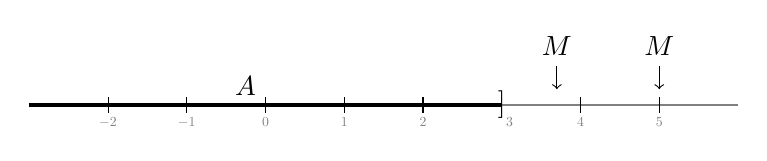
\begin{tikzpicture}
    \draw[gray] (-3, 0) -- (6, 0);


    %% drawing the set A
    \node[above left] at (0,0) {\(A\)};
    \node at (3,0) {\(]\)}; 
    \draw[very thick] (-3,0) -- (3,0);
    
    %% drawing M
    \draw[<-] (5,0.2)--(5,0.5) node[above]{\(M\)};
    \draw[<-] (3.7,0.2)--(3.7,0.5) node[above]{\(M\)};

    %% tick
    \foreach \i in {-2,-1,0,1,2, 4, 5}{
      \draw (\i, -0.1) -- (\i, 0.1)
      node[below=2mm , scale=0.5, color=gray]{\(\i\)};}
    \draw (3, -0.1) -- (3, 0.1)
    node[right = 1mm,below=2mm,scale=0.5, color=gray]{\(3\)};
    
  \end{tikzpicture}
\end{center}

So whenever we talk about set that is bounded above, you are encouraged to
picture it just like the one above. Below, we give the formal definition

\begin{definition}[Bounded above]
  Let \(A\subset\R\) and \(M\in\R\).
  \begin{itemize}
  \item
    We say that \(M\) is an \emph{upper bound} of \(A\) if
    \(\forall a\in A, a\leq M\).
  \item
    We say that the set \(A\) is \emph{bounded above}
    if \(A\) has an upper bound; in symbol we mean
    \(\exists M\in\R,~\forall a\in A,~a\leq M\).
  \end{itemize}
\end{definition}

Similarly, there is a notion of bounded below and the notion of
lower bound. Imagine the set \(A\) and a number \(m\) as below.

\begin{center}
  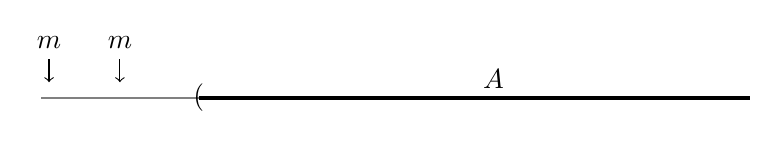
\begin{tikzpicture}
    \draw[gray] (-3, 0) -- (6, 0);

    %% drawing the set A
    \node[above left] at (3,0) {\(A\)};
    \node at (-1,0) {\((\)}; 
    \draw[very thick] (-1,0) -- (6,0);
    
    %% drawing m
    \draw[<-] (-2,0.2)--(-2,0.5) node[above]{\(m\)};
    \draw[<-] (-2.9,0.2)--(-2.9,0.5) node[above]{\(m\)};
  \end{tikzpicture}
\end{center}

\begin{definition}[Bounded below]
  Let \(A\subset\R\) and \(m\in\R\).
  \begin{itemize}
  \item
    We say that \(m\) is a \emph{lower bound} of \(A\) if
    \(\forall a\in A, a\geq m\).
  \item
    We say that the set \(A\) is \emph{bounded below}
    if \(A\) has a lower bound; in symbol we mean
    \(\exists m\in\R,~\forall a\in A,~a\geq m\).
  \end{itemize}
\end{definition}

Don't memorise the definition! Try to imagine them as pictures in your
head, and formulate which one is smaller, which one is bigger.
To better understand the definition, we need to pracise with some examples.

\begin{example}
  The set \(A = (-\infty, 3]\) is bounded above. To prove this, we
  need to choose a number \(M\) that is an upper bound of \(A\).
  There are a lot of choices of \(M\), so any one of them is fine. Here
  we decided to choose choose \(M=5\) and we see that
  \(\forall a\in A\) we have \(a\leq 3< M\).
  Therefore \(A\) is bounded above.
\end{example}

\begin{example}
  Let \(A = (-1, 3]\). Is \(M=2.8\) an upper bound of \(A\)?
  Looking at the picture, it seems that \(M\) is \emph{not}
  an upper bound of \(A\).
\end{example}

\begin{center}
  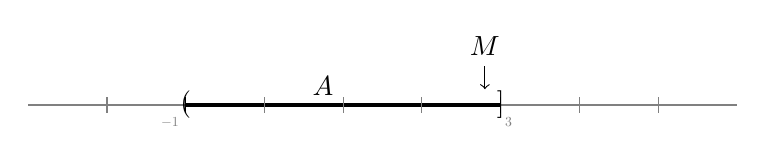
\begin{tikzpicture}
    \draw[gray] (-3, 0) -- (6, 0);

    %% drawing the set A
    \node[above left] at (1,0) {\(A\)};
    \node at (-1,0) {\((\)}; 
    \node at (3 ,0) {\(]\)}; 
    \draw[very thick] (-1,0) -- (3,0);
    
    %% drawing M
    \draw[<-] (2.8,0.2)--(2.8,0.5) node[above]{\(M\)};

    %% tick
    \foreach \i in {-2,0,1,2, 4, 5}{
      \draw[gray] (\i, -0.1) -- (\i, 0.1);}
    \draw (3, -0.1) -- (3, 0.1)
    node[right = 1mm,below=2mm,scale=0.5, color=gray]{\(3\)};
    \draw (-1, -0.1) -- (-1, 0.1)
    node[left = 2mm,below=2mm,scale=0.5, color=gray]{\(-1\)};
  \end{tikzpicture}
\end{center}
Since we are not a kid anymore, we need to prove this using
the definition. But, what does it mean for \(M=2.8\) not an upper bound?
Think about it with the analogy this way:
\begin{itemize}
\item less than or equals to = obey
\item \(2.8\) is upper bound if every numbers in \(A\) has to obey \(2.8\).
\item So if \emph{there is} some numbers is \(A\) that doesn't obey \(2.8\),
  then we can conclude that \(2.8\) is no longer an uppper bound, i.e.
  \[ 2.8 \text{ not uppper bound } \iff \exists a\in A,~ a>2.8\]
  In general,
  \fbox{\(M\) is \emph{not} upper bound of \(A\) if \(\exists a\in A, a>M.\)}
  This is called negating the definition. It is a good pracise
  for you to negate a definition whenever you encounter one.
\end{itemize}
Now, back to our example when \(A = (-1, 3]\) and \(M=2.8\).
We can see now that \(2.8\) is not an upper bound since
there is an element \(a = 2.99\in A\) such that \(a>M\).
Note that we can choose a different \(a\) as long as it is in \(A\)
and bigger than \(M\). For example we can instead choose
\(a=2.81\) or \(2.9\) or \(2.992024\) or even \(3\), et cetera.


\begin{example}
  Let \(A = (3, +\infty) = \{x\in\R\colon x> 3\}\).
  Is this set bounded above?
  Drawing the pictures, you will see that elements of \(A\)
  go forever to the right, which means that \(A\) is not bounded above.
  Again, we are no longer a kiddo. We need to prove this assertion
  using a definition. Now, what does it mean to be unbounded above?
  We need to negate the definition!
  \begin{itemize}
  \item \(A\) is bounded above means: \(A\) has an upper bound.
  \item So \(A\) is unbounded above means: \(A\) doesn't have an upper bound.
    To be more precise, this means that any number \(M\in\R\),
    this number is never ever an upper bound of \(A\).
    We get the following.
    \begin{align*}
      A \text{ unbounded above}
      &\iff A \text{ has no upper bound}\\
      &\iff \forall M\in\R,~M \text{ is not an upper bound of } A\\
      &\iff \boxed{\forall M\in\R,~\exists a\in A,~ a>M.}
    \end{align*}
  \end{itemize}
  Let's imagine the boxed statement as a game between you and me.
  The game goes as follow: I give you a number \(M\),
  you must respond by choosing a number \(a\in A\) that is bigger than \(M\).
  Ready?
  \begin{itemize}
  \item If I give you \(M=10\), what is your response? Well, you have
    a lot of response! You can choose \(a=11\) or \(12\) or \(10.1291\).
    These numbers are all in \(A\) and are bigger than \(M\).
  \item If I give you \(M=100\), you can response by simply choosing \(a=101\).
  \item In the end, you need to have a formula, this formula could tell
    you what to respond to my challenge \(M\).
  \item If I give you \(M\) in general, what is your response?
    Some of you might think of the response \(a=M+1\).
    This is fine if the value \(M\) is larger than \(3\).
  \item If I give you \(M=1\), then the response \(a=M+1\) is no longer valid,
    because now \(a=2>M\) but \(a\notin A\).
    But this is easily fixed. If I give you any \(M>3\),
    you could choose the response \(a = M+1\). But if I give you \(M\leq 3\),
    you can response by choosing \(a=4\in A\).
  \end{itemize}
  Now we prove that the set \(A = (3,+\infty)\) is unbounded above.
  Let \(M\in\R\) be an arbitrary number, now
  \begin{itemize}
  \item if \(M\geq 3\), we choose \(a=M+1\). We see that \(a>M\), and also
    \(a\in A\);
  \item if \(M<3\), we choose \(a = 4\). We see that \(a>M\) and \(a\in A\).
  \end{itemize}
  In both cases we get, \(\forall M\in\R,\exists a\in A,a>M\).
  Therefore, \(A\) is unbounded above.

\end{example}


% \newpage
% \subsection{Relation between \(\N\) and \(\R\)}
% Here we assume that there exists \(\N\) a subset of \(\R\) with the following
% properties:
% \begin{enumerate}[label = {(\roman*).}]
% \item \(1\in\N\), and is the smallest element in \(\N\);
% \item If \(n\in\N\), then \(n+1\in\N\);
% \item If \(n,m\in\N\) such that \(n\neq m\), then
%   \(\abs{n-m}\geq 1\).
% \end{enumerate}

% \begin{theorem}[Archimedean Property]
%   The set \(\N\) is not bounded above. In other words,
%   for any \(x\in\R\), there exists \(n\in\N\) such that \(n>x\). 
% \end{theorem}
% \begin{proof}
%   Assume by contradiction that the above statement is wrong, that is
%   the set \(\N\) is bounded above.
%   Thus \(\alpha = \sup\N\) exists. By definition of supremum,
%   there is \(n\in\N\) so that
%   \[
%     n > \alpha - 1 \implies \alpha < n+1.
%   \]
%   However, this is a contradiction since \(n+1\in\N\) and \(\alpha\)
%   is supposed to be an upper bound of \(\N\).
% \end{proof}

% \begin{theorem}[Well-ordering property]
%   Any non-empty subset \(S\subset\N\) has a minimal element;
%   in other words \(\min S\in S\).
% \end{theorem}
% \begin{proof}
%   Let \(S\subset\N\) and \(S\neq\varnothing\). Since \(\N\) bounded below,
%   then so does \(S\). We conclude from completeness property that
%   \(\alpha = \inf S\in\R\) exists.
%   It suffices to prove that \(\alpha \in S\). Argue by contradiction and
%   suppose that \(\alpha\notin S\). In particular, \(\alpha\) is an a natural
%   number.
%   %
%   From definition of infimum, there is an element \(s\in S\) so that
%   \(\alpha \leq s<\alpha+1  \).
%   Moreover we cannot have \(\alpha=s\), since we assumed \(\alpha\notin S\).
%   Thus we have found \(s\in S\) such that
%   \[\alpha<s<\alpha+1.\]
%   Notice that \(s\) is a number that is greater than \(\alpha=\inf S\).
%   Using definition of infimum again, we conclude that there is
%   \(s'\in S\) with \(\alpha \leq s' < s\). Using the same argument as above,
%   we must have \(\alpha < s'\). Combining all inequalities, we obtain
%   \[\alpha < s' < s < \alpha+1. \]
%   Hence \(0< s-s' <  1\). This is a contradiction to the (iii) property
%   of \(\N\).
% \end{proof}



% \subsection{Relation between \(\Q\) and \(\R\)}

% \begin{theorem}[Density of \(\Q\) in \(\R\)]
%   For any two distinct real numbers \(x,y\in\R\) with \(x<y\),
%   there is a rational number \(r\in\Q\) satisfying
%   \(x<r<y\).
% \end{theorem}
% We say that a set \(A\subset\R\) is dense provided that
% for any \(x<y\), there exists \(a\in A\) with \(x<a<y\).
% From the above theorem, the set \(\Q\) has this exact property.
% In other words, this means that no matter how you choose \(x\) and \(y\),
% there is always an element in \(\Q\) sits between them.
% Visually, the elements of \(\Q\) are densely put into \(\R\),
% that is why we say \(\Q\) is dense in \(\R\).

% The machinery of the proof is to use Archimedean property.
% To shorten the proof a bit, we are going to use the fact that,
% for any two numbers that are strictly of distance 1 apart,
% there is an integer sits between them. This fact is left as
% an exercise, as you can see in
% \href{https://sivmeng.com/real-analysis-2425/td/td1.pdf}{\sffamily TD n\textdegree 1}.

% \begin{proof}
%   Let \(x<y\) be real numbers. From Archimedean property,
%   there is an natural number \(n\in\N\) such that \(n>\frac{1}{y-x}\).
%   Equivalently,
%   \[ny - nx >1.\]
%   Since \(ny\) and \(nx\) are strictly of distance 1 part,
%   there is an integer \(m\in\Z\) such that \(nx<m<ny\).
%   Thus
%   \[x < \frac{m}{n} < y.\]
%   Therefore, we have found a rational number \(\frac{m}{n}\)
%   that is between \(x\) and \(y\). This concludes the proof.
% \end{proof}






\end{document}
